\begin{thebibliography}{9}

\bibitem{gert001}
	Malene(0 - 21:03), Gert(21:03 - 1:13:20) \& Lasse(1:13:20 - slut).3ga - Time 24:47\\
	\textit{[...] vi henter jo hver dag nede i Holland og leverer i hele Danmark inden 7.}

\bibitem{gert002}
	Malene(0 - 21:03), Gert(21:03 - 1:13:20) \& Lasse(1:13:20 - slut).3ga - Time 43:00\\
	\textit{[...] hente nede i Salzgitter som ligger nede syd for Hannover klokken 15:30 og så samtidig levere oppe nord for Stockholm inden 7 næste morgen.}

\bibitem{gert003}
	Gert \#2 2/2.3ga - Time 02:17\\
	\textit{[...], så skal man altså også have løsningsdelen med, hvornår det er løst og sådan, før det har en værdi der. Og hvis man ikke gør det, så føler jeg at det mister meget af sin værdi.}

\bibitem{gert004}
	Gert \#2 1/2.3ga - Time 03:10\\
	\textit{[...] og hvis de ringer til vores hovednummer er det control tower de får, så det er jo egentlig der den meste kontakt foregår}

\bibitem{gert005}
	Gert \#2 1/2.3ga - Time 04:15\\
	Om kontroltårnet selv løser problemer for kunder: \textit{Det kunne sagtens være, der hvor kunden siger noget, kan vi godt sige til dem, jamen prøv at hør, hvis du nu går ind på vores hjemmeside, så kan du gøre sådan og sådan}

\bibitem{gert006}
	Gert \#2 1/2.3ga - Time 06:21\\
	\textit{Hvis jeg får noget fra en intern eller en kunde prøver jeg på en eller anden måde at oversætte det sådan at det er mere klart defineret når det kommer til IT}

\bibitem{gert007}
	Gert \#2 1/2.3ga - Time 03:30\\
	\textit{\emph{(rd: om kunden)} som så skyder det ind på et andet niveau her, for eksempel ved at kontakte mig eller Bob, eller et andet niveau altså}

\bibitem{gert009}
	Gert \#2 1/2.3ga - Time 14:45\\
	Om de får den samme support request flere gange: \textit{Hvis du får den samme forespørgsel flere gange så er det jo en rykker, enten fordi vi snakkede om det dengang eller fordi vi ikke lige har fået set på det, og det så bliver nævnt igen. Også siger vi jo det skal vi nok prøve at se på eller komme tilbage til også er vi ikke lige kommet tilbage.} Interviewer: \textit{Hvad er årsagen til det?} \textit{Det er fordi hvis jeg sender en mail til Lasse så er det ikke sikkert jeg husker at følge op på det, og hvis han ikke svarer, så husker jeg det først når kunden rykker på mig, så vi mangler et struktureringsværktøj. }

\bibitem{gert010}
	Malene(0 - 21:03), Gert(21:03 - 1:13:20) \& Lasse(1:13:20 - slut).3ga - Time 1:08:10\\
	Interviewer: \textit{Kan du fortælle lidt om ESLA?}\\
	Gert: \textit{Ja og det er også det partnerskab vi har, det er ESLA.}\\
	\textit{[...] Vi går ud og markedsfører og sammen og hvis vi får en kunde der vil bruge den samme, jamen så kan vi snart gå ud og dække en stor del af Europa med det samme tilbud.}\\
	\textit{[...] og bruge hinanden også har meget, vi vil være gode venner og vi supporter hinanden hvis der er et eller andet vi kan hjælpe hinanden med det gør vi meget for at gøre. Har meget open books, de må gerne komme op og se alt hvordan vi producerer, jeg må gerne komme ned og se hvordan de producerer, jeg har så ikke fået gjort det endnu.}

\bibitem{gert011}
	Gert \#2 1/2.3ga - Time 18:05\\
	Interviewer: \textit{Har i egentlig nogen KPIer i forhold til svartider?}\\
	Gert: \textit{Nej, slet ikke, overhovedet ikke. Det har vi ikke.}

\bibitem{gert012}
	Gert \#2 1/2.3ga - Time 18:20
	Om customer support:
	\textit{Vi har ingen form for dokumentation på det.}

\bibitem{gert013}
	Gert \#2 1/2 - Time 21:11
	\textit{Nu her er vi blevet bekræftiget i at vi skal starte en stor kunde op i danmark og sverige og de skal starte her den første januar, jamen så integrerer vi til den første januar.}

\bibitem{gert014}
	Telefonopkald med Gert\\
	Interviewer: \textit{Ved du ca. hvor mange der arbejder i operationen?}
	 Gert: \textit{I operationen og i control tower er der seks mennesker.}

\bibitem{gert015}
	Telefonopkald med Gert\\
	Interviewer: \textit{Ser du en af dine primære interesser, som at være optimering af operationen?} Gert: \textit{Ja, helt klart.}

\bibitem{gert016}
	Telefonopkald med Gert\\
	Interviewer: \textit{Ser du en af operationens interesser som at være at give effektiv customer support?} Gert: \textit{Ja, det tror jeg også at jeg vil sige ja til.}

\bibitem{gert017}
	Gert \#2 1/2.3ga - Time 10:06\\
	\textit{Jamen, egentlig har det været it@, men nu har de delt dem op og de har også lavet en der hedder support@danx.dk og development, vi har bare ikke spredt rygtet om det endnu, og vi har faktisk haft et møde i dag om med de forskellige operationschefer i de forskellige lande, hvor vi havde lasse med inde for at få noget struktur over det. [...] Så det er klart at der skal være en mail kun til dem og den er vist også ved at blive fabrikeret og publiceret. }

\bibitem{gert018}
	Malene(0 - 21:03), Gert(21:03 - 1:13:20) \& Lasse(1:13:20 - slut).3ga - Time 25:50\\
	\textit{Under høsten der er det jo sådan at en landmand, der ser vejrudsigten, “nu er det altså i morgen jeg skal høste”, også ryger kniven på hans mejetærsker, så vil han altså have den ud og køre i morgen}

\bibitem{gert019}
	Gert \#2 1/2.3ga - Time 08:41\\
	\textit{Jeg sidder jo her hvor jeg sidder, så nogle gange går jeg ind til ham\emph{(rd: Lasse)}, nogle gange sender jeg en mail, og det er ret sjældent jeg ringer til ham.}

\bibitem{gert020}
	Gert \#2 1/2.3ga - Time 12:54\\
	Interviewer: \textit{Hvis du kunne lave et skøn, de henvendelser I får fra kunden som ikke er fra statusmøder, hvor mange af dem er skriftlige og hvor mange af dem er mundtlige?} Gert: \textit{Der vil jeg tro at langt de fleste er skriftlige.}

\bibitem{gert021}
	Malene(0 - 21:03), Gert(21:03 - 1:13:20) \& Lasse(1:13:20 - slut).3ga - Time 29:21\\
	Interviewer: \textit{Jeg kunne forstå i bruger fly udelukkende til blandt andet Helsinki, har i så samarbejde med flyselskaberne sådan at i sikrer at der er plads til jeres var der skal leveres}\\
	\textit{[..] Fly selskaber vil primært transportere passagere, så uanset hvad vil der indgå en situation hvor et fly er sent på den, og så siger kaptajnen, for han vil gerne flyve til tiden, så siger han, vi tager ikke noget fragt med i dag.}

\bibitem{gert022}
	Malene(0 - 21:03), Gert(21:03 - 1:13:20) \& Lasse(1:13:20 - slut).3ga - Time 50:47\\
	Interviewer: \textit{Vi er interesseret i at vide noget om jeres struktur, hvilke afdelinger i har og hvordan de snakker sammen.}\\
	Gert: \textit{Hvert land har en landechef, hvert land har også en ansvarlig for operationen, og hvert land har faktisk også, undtagen Norge, en sælger, altså en der er tilknyttet vores salgsafdeling. Og det er jo klart at det er landecheferne der er ansvarlige for at deres land fungere både operationelt og administrativt og med legale, personale og alt sådan noget der og salgsmæssigt. Og så har vi alligevel valgt at have en nordisk operationsafdeling som jeg så leder [..] Så har vi en nordisk salgsafdeling. [..] Vores IT er nordisk og ligger her i vallenspæk. }

\bibitem{gert023}
	Malene(0 - 21:03), Gert(21:03 - 1:13:20) \& Lasse(1:13:20 - slut).3ga - Time 41:59\\
	Gert: \textit{PUDO’er er sådan en ting, som er customer driven, altså kundernes behov, altså det der har fået os til at åbne måske 28 PUDO’er i sverige er fordi IBM vil have PUDO’er og HP vil have PUDO’er og [Bincoy Neksdov] vil have PUDO’er, så åbner vi alle de der PUDO’er i sverige. Så det er jo klar, det er også med til at styrke os. Og nu er det så vigtigt for os at få flere kunder ind på PUDO’erne, for sådan nogle PUDO’er har typisk en fast månedlig omkostning. Som helst skal være så lille så muligt, og alligevel skal vi have så meget så muligt gennem PUDO’erne.}

\bibitem{gert024}
	Telefonopkald med Gert\\
	Interviewer: \textit{Har alle der giver customer support deres egen computer?} Gert: \textit{Ja, det har de.}

\bibitem{gert025}
	Malene(0 - 21:03), Gert(21:03 - 1:13:20) \& Lasse(1:13:20 - slut).3ga - Time 39:12\\
	Interviewer: \textit{Hvordan prøver i at adskille jer fra jeres konkurrenter? Altså hvorfor vælger kunden jer frem for en anden?} Gert: 	\textit{Der hvor vi prøver og altid har prøvet at stå lidt for os selv, det er at vi har en høj kvalitet og vi gør meget for at have en høj kvalitet.}

\bibitem{gert026}
	Malene(0 - 21:03), Gert(21:03 - 1:13:20) \& Lasse(1:13:20 - slut).3ga - Time 39:12\\
	Interviewer: \textit{Hvordan måles denne her branche sig på kvalitet?} Gert: 	\textit{Det er levering til tiden, og ved forsinkelser, årsagen til den.}

\bibitem{gert027}
	Malene(0 - 21:03), Gert(21:03 - 1:13:20) \& Lasse(1:13:20 - slut).3ga - Time 40:10\\
	Gert: \textit{[...] der vil aldrig nogensinde stå i en oplysning fra os til kunden at vores bil er punkteret for eksempel. Det kan godt være vi har et technical breakdown, men det er sjældent. Hvis vi har et problem og vi kan nå, ved at bruge nogle penge, og så stadig levere til tiden, så gør vi det. Så vi investerer meget backup omkostninger i at holde vores høje kvalitet.}

\bibitem{gert028}
	Malene(0 - 21:03), Gert(21:03 - 1:13:20) \& Lasse(1:13:20 - slut).3ga - Time 51:07\\
	Gert: \textit{Jamen, du kan sige, vi er en ret flad organisation. Vi har afdelinger i alle landene.}

\bibitem{bob001}
	\textit{Nogle potentielle kunder vil gerne se support KPIer.}

\bibitem{bob002}
	\textit{Nogle kunder kræver referencer fra andre kunder.}

\bibitem{bob003}
	\textit{Dvs at vi fokusere på at vokse med ca. 25-30 om året i organisk vækst \emph{(rd: nye kunder)}}\\
\textit{Sidst eår tjene vi ca 10 mill indne skal, hvilket er for lidt ud af 250 mill i omsætning. I indeværende år (13/14) kommer vil til at omsætte plus 300 mill og et overskud på plus 20 mill før skat.}\\
\textit{Overordnede sigter jeg mod at DANX om 3-4 år har en omsætning på plus 500 mill med et overskud på ca 8-10 procent. Det vil give en potentiel salgsværdig på + 500 mill.}

\bibitem{bob004}
	Hvor meget koster det ca. at implementere en ny kunde?
	\textit{“Jeg vil skyde på at det koster 15000 it-mæssigt, 40000 operationelt og 30000 salgsmæssigt.”}

\bibitem{malene001}
	Malene(0 - 21:03), Gert(21:03 - 1:13:20) \& Lasse(1:13:20 - slut).3ga - Time 09:23\\
	\textit{[...] nogen af vores største konkurrenter er TNT og HIT}

\bibitem{malene002}
	Malene(0 - 21:03), Gert(21:03 - 1:13:20) \& Lasse(1:13:20 - slut).3ga - Time 04:30
	\textit{Søren gønge, som er ham der grundlagde firmaet, er ham der ejer mest også har Bob også en stor del af aktierne, også alle tre country managers der sidder i norge, sverige og finland ejer også en del af virksomheden.}

\bibitem{opemployee001}
	\textit{“Vi har på nuværende tidspunkt en hel reol stående med ringbind til de 19 systemer som vi benytter i forbindelse med vores kundesystemer”}

\bibitem{lahib001}
	Lahib.3ga - Time 13:00\\
	\textit{[...] så jeg programmerede noget 3 måneder siden og fuldstændig glemt hvordan fanden jeg havde lavet det. Så jeg skulle gå helt tilbage og justere det eller faktisk skrotte det fuldstændig og lave noget helt ny implementering.}

\bibitem{lahib002}
	Lahib.3ga - Time 00:51
	\textit{Min opgave har så været, for 3-5 kunder at få forbindelse til en ftp eller en sftp server hvor jeg kan hente filerne, arkivere dem også bagefter uploadede dem, så det er både upload og download og arkivering af filerne.}

\bibitem{lahib003}
	Lahib.3ga - Time 17:42
	\textit{Hvorimod Lasse han har direkte kontakt med kunden, hvor kunden siger “Det her, jeg har seks filer der ikke er kommet i dag, hvad er der sket, de her filer er ikke blevet importeret fra vores til jeres server.” Så jeg vil sige, Lasse ja, og Jakob lidt, men mig og Safe vi får ikke så mange \emph{(rd: customer support requests)}.}

\bibitem{lahib004}
	Lahib.3ga - Time 17:09
	\textit{Lasse får sindsygt meget(support requests) hver dag. Jeg gør ikke, Safe gør heller ikke, Jakob gør lidt, mere end mig.}

\bibitem{lasse001}
	Lasse \#5.3ga - Time 15:25 \\
	Interviewer: \textit{Hvor ofte er operationen mellemled for support henvendelser fra kunden?} Lasse: \textit{Stort set altid, vi snakker 90\% af gangene i hvert fald}

\bibitem{lasse002}
	Lasse \#5.3ga - Time 8:27 \\
	Til om nogen fra operationen kan løse it-problemer: \textit{Det er igen lidt et tilfælde hvem der kan det og ikke kan det.}

\bibitem{lasse003}
	Lasse \#5.3ga - Time 16:08 \\
	\textit{Jeg har jo lidt et problem eller en udfordring med ved at vi har to afdelinger både en IT support og en IT development, og de sender jo bare til @it som har begge afdelinger blandet sammen så vi for jo en masse mails hvis der er for eksempel problemer med PDA’erne eller et andet hvor det sådan set ikke er min afdeling, så vi får en masse clutter-mail på grund af det her.}

\bibitem{lasse004}
	Lasse \#5.3ga - Time 17:10 \\
	\textit{Hvis de andre har travlt så svarer vi jo også, vi hjælper jo hinanden \emph{(rd: IT afdelingerne)}}

\bibitem{lasse005}
	Lasse \#5.3ga - Time 18:30 \\
	Interviewer: \textit{Hvor de(operationen) har korrespenderet med en kunde?} Lasse: \textit{Ja, men hvor de så også skriver hvad det er der er problemet.}

\bibitem{lasse006}
	Lasse \#5.3ga - Time 21:35 \\
	\textit{Jeg har jo lært for eksempel haydar\emph{(rd: ansat i operationen)} at gå ind at kigge i EDI filen hvis der er fejl advisering eller et eller andet så han kan gå ind og se for vi gemmer dem et bestemt sted og han er begyndt at kunne gennemskue de fleste af dem, altså se hvordan ser denne her forsendelse egentlig ud, så han har taget meget af det jeg har siddet og gennemtrawlet og se om de har sendt den her forsendelse gennem de rigtige kanaler, er den i vores fil og i så fald hvad er der så gået galt.}

\bibitem{lasse007}
	Malene(0 - 21:03), Gert(21:03 - 1:13:20) \& Lasse(1:13:20 - slut).3ga - Time 01:50:38
	\textit{Nogle gange kunne det være meget rart for mig at sige, prøv at se her hvor meget vi egentlig har lavet, og her kunne et ticket system jo være meget relevant.}

\bibitem{lasse008}
	Lasse \#5.3ga - Time 03:13 \\
	\textit{Hvis ikke IT integrationen er færdig, jamen så kører vi ud med pakkerne alligevel, altså så gør vi det uden. Så vi kan som regel integrere en ny kunde, hvis de er klar, inden for en til to dage.}

\bibitem{lasse009}
	Malene(0 - 21:03), Gert(21:03 - 1:13:20) \& Lasse(1:13:20 - slut).3ga - Time 02:05:38
	Om hvordan arbejdet bliver struktureret \textit{Vi holder møder, jeg holder ugentlige møder, nogen gange er det hver 14 dag eller en gang om måneden, det kommer lidt an på hvor meget stress der er på, men hvor at, altså vi har ikke noget task system eller management system, så det bliver meget lister, hvor jeg siger “nu vil jeg gerne have en liste på alt det der mangler i det her system” også sidder jeg og prioriterer hvad der er vigtigt og hvad der er knap så vigtigt.}

\bibitem{lasse010}
	Lasse \#2.3ga - Time 08:30\\
	\textit{[...] ofte så bruger folk ikke de der 5 minutter på at skrive en mail og skrive præcis hvad problemet er, så det ender med en mailkorrespondance på 5 mails frem og tilbage, for at finde ud af hvad problemstillingen er.}

\bibitem{lasse011}
	Lasse \#2.3ga - Time 20:10\\
	\textit{Jeg har snakket med i hvert fald 10 og det var kun inden for IT området, altså der var også alt det praktiske. Der er det jo smart at der er 10 mennesker der kan snakke med mig, altså jeg ved alt det 10 mennesker ved på deres side.}

\bibitem{lasse012}
	Malene(0 - 21:03), Gert(21:03 - 1:13:20) \& Lasse(1:13:20 - slut).3ga - Time 01:18:32
	\textit{Jeg synes det fungerer rigtigt godt, jeg synes vi har en fordel i forhold til nogle af de andre firmaer, at de\emph{(rd: kunder)} kan komme i kontakt til os direkte, at vi ikke har et support system og et 4 tiers call desk hvor at man skal igennem de første tre der ikke ved noget som helst, som nogle af vores konkurrenter har, og det er en fordel, og det ser vores kunder helt klart også som en fordel.}

\bibitem{lasse013}
	Lasse \#5.3ga - Time 10:00 \\
	Interviewer: \textit{På ugentlig basis hvor ofte bruger du så mere end 2 minutter på at finde ud af hvilken kunde en mail kommer fra.} Lasse: \textit{Måske, gennemsnitlig 2-3 gange om ugen.} Interviewer: \textit{Hvor lang tid bruger du på det?} Lasse: \textit{ti minutter, et kvarter.}

\bibitem{lasse014}
	Malene(0 - 21:03), Gert(21:03 - 1:13:20) \& Lasse(1:13:20 - slut).3ga - Time 01:14:07
	\textit{Jeg står for udviklingen her}
 
\bibitem{lasse015}
	Malene(0 - 21:03), Gert(21:03 - 1:13:20) \& Lasse(1:13:20 - slut).3ga - Time 01:14:20
	\textit{Vi har jo en masse systemer internt kørende og vi har jo vores eget udvikling trackit}

\bibitem{lasse016}
	Malene(0 - 21:03), Gert(21:03 - 1:13:20) \& Lasse(1:13:20 - slut).3ga - Time 01:18:13
	\textit{jeg bruger også uendelig meget tid på mail og telefon korrespondancer med både vores egne medarbejdere men også vores kunder}

\bibitem{lasse017}
	Lasse \#5.3ga - Time 14:52 \\
	Interviewer: ``Du får nogle kunde problem henvendelser fra Gert, fra operationen?’’
Lasse: \textit{Ja}

\bibitem{lasse018}
	Malene(0 - 21:03), Gert(21:03 - 1:13:20) \& Lasse(1:13:20 - slut).3ga - Time 01:14:35
	Med hensyn til hvad Lasse laver: \textit{handler meget om integration af vores kunder}

\bibitem{lasse019}
	Malene(0 - 21:03), Gert(21:03 - 1:13:20) \& Lasse(1:13:20 - slut).3ga - Time 01:15:40
	I forbindelse med kunders systemer i pudo: \textit{... og så bruger vi en masse af kundens systemer, så hvis du tæller dem med altså det er jo som regel de her hjemmesider som de logger ind på fordi at de skal ind på vores kunders lager databaser...}

\bibitem{tnt001}
	Interviewer: \textit{Hvor lang tid tager det typisk at integrere en ny kunde?}
	TNT: \textit{En typisk kunde med ca. 20 servicevogne tager 14 dage at integrere.}

\bibitem{tnt002}
	http://www.tnt.com/express/da\_dk/site/home/Om\_TNT/om\_tnt.html

\bibitem{bank001}
	Interviewer: \textit{Hvilken rente kan en mellemstor virksomhed få, forudsat de har ca. 50 millioner stående og pengene ikke må være låst?}\\
	Bank: \textit{Op til én million får de 0.775\%, derefter får de mellem 0\% og 0.125\%.}

\bibitem{webpage001}
	http://www.tnt.com/express/da\_dk/site/home/vores\_services/TNT\_innight.html

\bibitem{webpage002}
	http://www.postnordlogistics.dk/da/Sider/hit.aspx

\bibitem{webpage003}
	http://www.posten.se/en/Logistics/InNight/Pages/home.aspx

\bibitem{webpage004}
	http://www.fedex.com/dk/shipping-services/domestic/

\bibitem{webpage005}
	http://www.kayako.com/

\bibitem{webpage006}
	http://www.kayako.com/company/customers/

\bibitem{webpage007}
	http://www.g2crowd.com/survey\_responses/kayako-fusion-review-10500

\bibitem{webpage008}
	http://www.kayako.com/signup/download/case/

\bibitem{webpage009}
	http://wiki.kayako.com/display/DOCS/Kayako+Query+Language+(KQL)

\bibitem{webpage010}
	http://danx.dk/Info/Profile

\bibitem{webpage011}
	https://www.fedex.com/ratefinder/home?source=gh\&cc=dk\&language=da

\bibitem{webpage012}
	http://www.postnordlogistics.dk/da/om-postnord-logistics/Sider/home.aspx

\bibitem{mail}
	\textit{The following is a mail recieved from Bob Thorhauge.}\\
	Vi har generelt en vækst strategi. Se evt power point vedhæftet. Dvs at vi fokusere på at vokse med ca. 25-30 om året i organisk vækst \emph{(rd: nye kunder)}. I indeværende regnskabsår sætter vi også fokus på vores indtjening. Sidste år tjente vi ca 10 mill inden skat, hvilket er for lidt ud af 250 mill i omsætning. I indeværende år (13/14) kommer vil til at omsætte plus 300 mill og et overskud på plus 20 mill før skat.\\
	Overordnede sigter jeg mod at DANX om 3-4 år har en omsætning på plus 500 mill med et overskud på ca 8-10 procent. Det vil give en potentiel salgsværdig på + 500 mill.\\
	Det er vores egentlig målsætninger. De andre ting er mere værdier for os. Vi arbejder med nedenstående values i virksomheden:
\begin{description}
\item[Reliability]
We have the integrity to keep our promises, to correct our mistakes and proactively inform our customers.
\item[Equality]
We are all equals, performing different roles to achieve the same goal.
We treat our customer, partners and colleagues with the same respect that we want to achieve ourselves.
\item[Quality]
We never take our customers for granted.
We strive for 100\% in everything we do – in that way we ensure that our customers live up to their customers’ high expectations.
\item[Flexibility]
Flexibility is our mindset. It is what we are and what we expect from all our employees and partners - nothing less.
\item[Creativity]
As pioneers we think out of the box and create solutions for our customers’ needs.
We are never satisfied and are constantly looking for new ways to improve.
\item[Availability]
We ensure our customers’ availability of spare parts through each employee’s personal care and availability.
\item[Pride]
We are proud of our customers, our company and our people - we take pride in everything we do.
\end{description}
Bob Thorhauge

\bibitem{img001}
	Slide from a DANX presentation\\
	%http://i.imgur.com/VcV07XS.png
	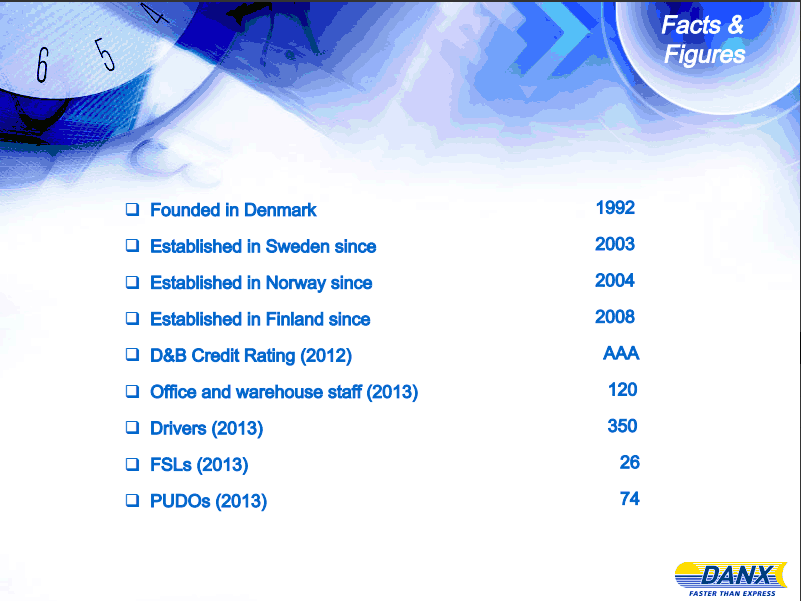
\includegraphics[scale=0.62]{img/DANX_FSL_PUDO}

\bibitem{img002}
	Cost benefit for tailored basic solution\\
	%http://i.imgur.com/rJZnQZi.png
	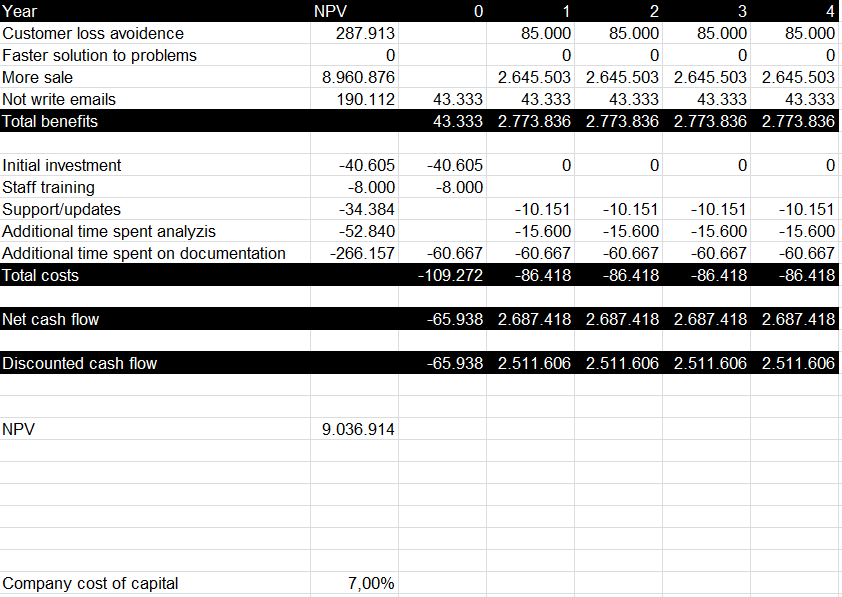
\includegraphics[scale=0.6]{img/CostBenefit_TailoredBasic}

\bibitem{img003}
	Cost benefit for tailored extended system\\
	%http://i.imgur.com/iNIannt.png
	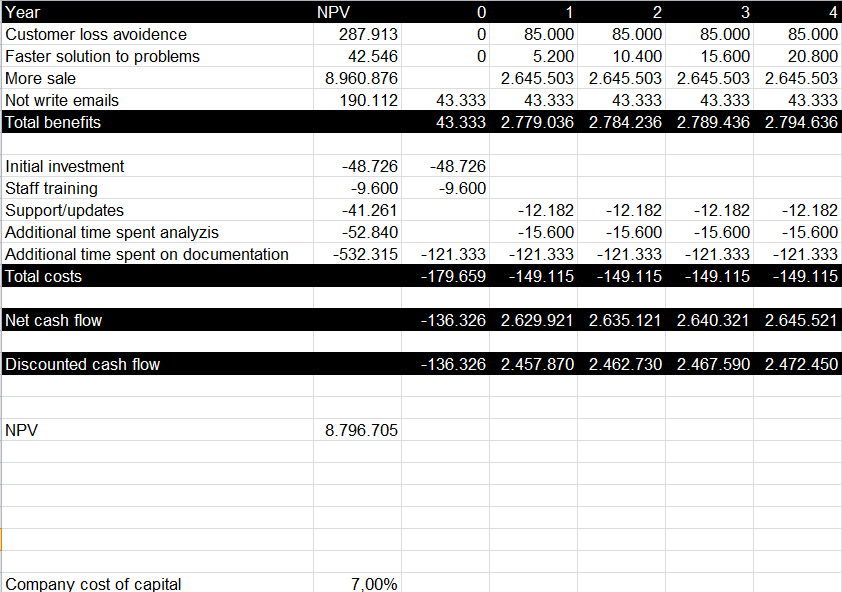
\includegraphics[scale=0.6]{img/CostBenefit_TailoredExtended}

\bibitem{img004}
	Cost benefit for off-the-shelf solution kayako\\
	%http://i.imgur.com/bUaRjPM.png
	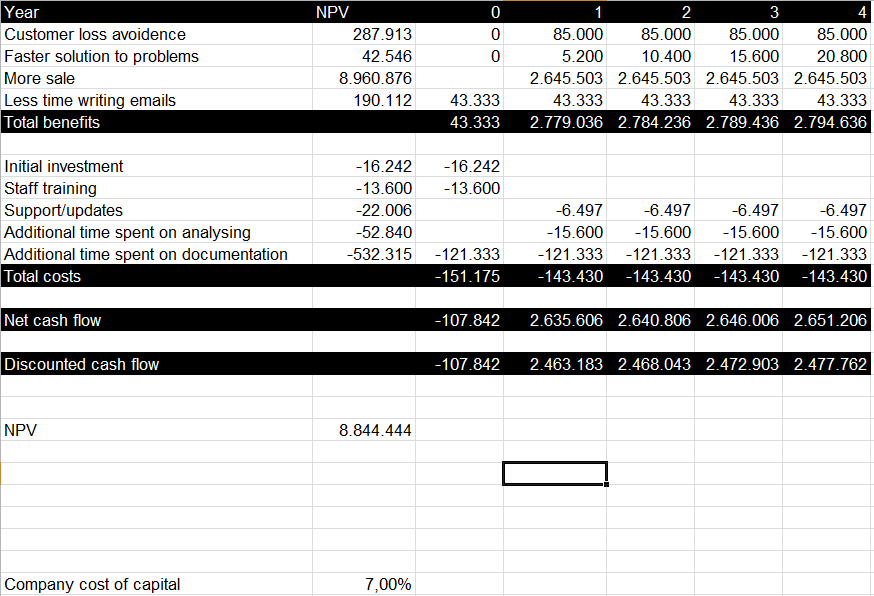
\includegraphics[scale=0.6]{img/CostBenefit_Off-the-shelf}

\end{thebibliography}
